\chapter{GUI}

\begin{center}
  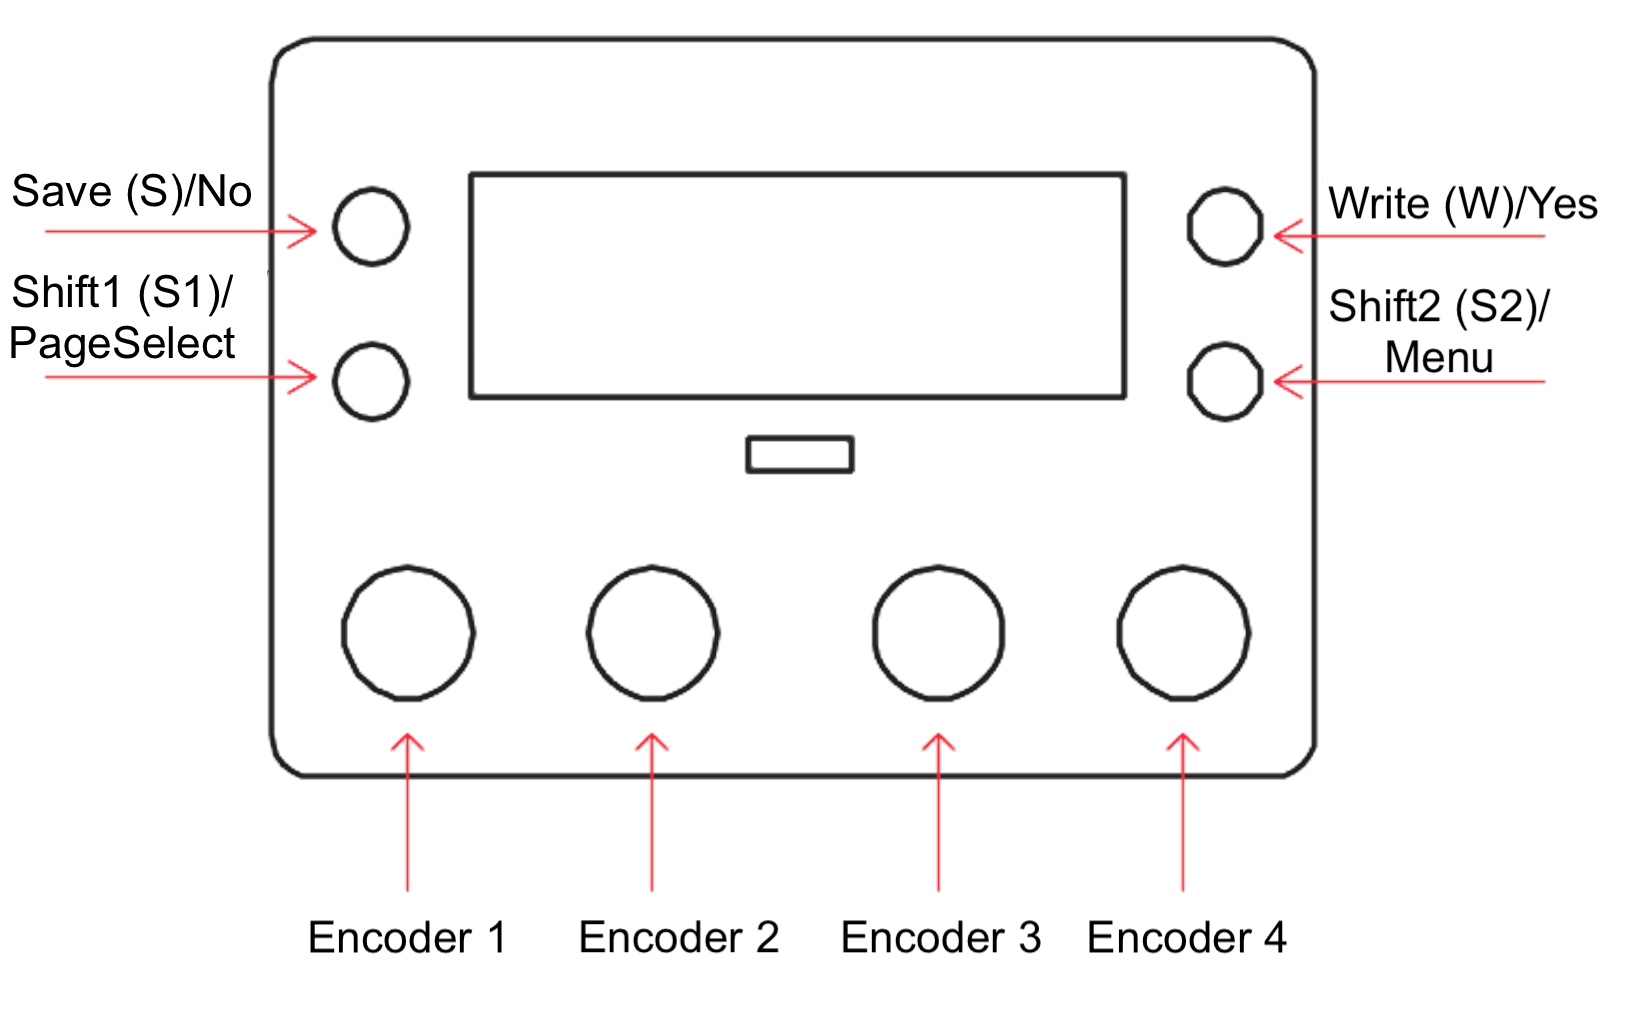
\includegraphics[width=16cm]{MC_Legend.png}
\end{center}

The MegaCommand's four upper function buttons are used to enter sub-menus and activate commands:
\section{Function Buttons:}
From the Grid Page the function buttons perform the following actions:
\begin{itemize}
\item{\textbf{[Save | No]}: Enters the Save Page}
\item{\textbf{[Write | Yes]}: Enters the Chain page}
\item{\textbf{[Shift1 | PageSelect]}: Enters the PageSelect page}
\item{\textbf{[Shift2 | Menu]}: Opens the slot Menu }
\end{itemize}
Combined Button Presses:
\begin{itemize}
\item{\textbf{[Save | No] + [Write | Yes]}: Opens the Global Settings menu }
\end{itemize}

\section{Encoder Buttons}
Encoder buttons are used to increase the speed of parameter rotation.
Holding down an encoder button whilst rotating the encoder will increase the update speed by 4x.

\section{Trigger Interface}
When connected to the Elektron MachineDrum, MCL will use the Machinedrum's 16 trigger buttons as additional GUI input. \\
\\
If connected to the Elektron AnalogFour (A4), MCL will use the A4's mini keyboard buttons as additional GUI input. Notes C,D,E,F are used to select A4 tracks 1,2,3,4 respectively.\\
\\
The Trigger Interface (TI) has different uses depending on the current page.\\
\\For example, the TI can be used to enter sequencer data in to the internal sequencer;
to select multiple tracks on the Mixer page and attenuate their volume simultaneously; to save or load Grid Slots from the Save or Chain pages and much more.

\subsection{MD Trigger Interface Limitations}
The MD TI is not natively supported by the MD and is instead achieved using a Global Slot/MIDI Channel exploit. The exploit is used to allow the user to press trigger buttons without triggering internal sounds. It also differentiate between notes triggered by the sequencer and notes triggered by a user key-press.\\
\\
The TI will cease working whenever the MD display is updated unexpectedly, for example, when a machine parameter's value is changed; or when a sub-menu on the MD is opened.\\
\\
As a precaution, whenever entering a Page on the MC that uses the TI, the MD's current track will automatically change to a track without Parameter locks. This avoids unexpected display updates that may be caused by transmitted Parameter Changes. If all tracks have parameter locks, then Track 16 will be chosen.\\
\\
\textit{Recovery: If the Trigger Interface stops working, exit and then re-enter the current page.}


